\documentclass[11pt, a4paper]{awesome-cv}
\geometry{left=1.8cm, top=1cm, right=1.8cm, bottom=1.5cm, footskip=.5cm}
\fontdir[fonts/]

\usepackage{pgfplots}
\usepackage{tikz}
\usepackage{pagecolor}
\usepackage{afterpage}
\usetikzlibrary{positioning, shapes.geometric, arrows.meta, calc}
\pgfplotsset{compat=1.18}

% Terminal dark theme colors
\definecolor{darkbg}{RGB}{12,12,12}
\definecolor{termgreen}{RGB}{51,255,51}
\definecolor{termgreendim}{RGB}{26,138,26}
\definecolor{termcyan}{RGB}{0,204,170}
\definecolor{termorange}{RGB}{255,107,53}
\definecolor{termwhite}{RGB}{232,232,232}
\definecolor{termgray}{RGB}{102,102,102}
\definecolor{termdarkgray}{RGB}{42,42,42}

% Set dark background
\pagecolor{darkbg}

% Override awesome-cv colors for dark theme
\colorlet{awesome}{termgreen}
\colorlet{text}{termwhite}
\colorlet{graytext}{termgray}
\colorlet{lighttext}{termgray}
\colorlet{darktext}{termwhite}
\colorlet{sectiondivider}{termgreendim}

% Configure hyperlinks
\hypersetup{
    colorlinks=true,
    linkcolor=termgreen,
    urlcolor=termgreen,
    citecolor=termgreen
}

\name{David H.}{Silver}
\position{Academy {\enskip$\rightarrow$\enskip} Industry {\enskip$\rightarrow$\enskip} Commercialization}
\address{NY, USA}
\mobile{+1-929-782-2060}
\email{david@embino.com}
\homepage{embino.com}
\linkedin{davidsilveril}

\begin{document}

\makecvheader

%%%%%%%%%%%%%%%%%%%%%%%%%%%%%%%%%%%%%%%%%%%%%%%%%%%%%%%%%%%%%%%%%%%%%%%%%%%%%%%
% PAGE 1 — CURRICULUM VITAE
%%%%%%%%%%%%%%%%%%%%%%%%%%%%%%%%%%%%%%%%%%%%%%%%%%%%%%%%%%%%%%%%%%%%%%%%%%%%%%%

\cvsection{Current Venture: Embino}
\begin{cvparagraph}
\href{https://embino.com}{embino.com} — Founder \& Inventor \hfill \textit{\color{termcyan}Stealth mode}

Natural-language programming for embedded devices. A grammar-constrained small language model generates verified bytecode that runs on ESP32, Arduino, RP2040, and any \$1 microcontroller. No hallucinations, no cloud dependency, deterministic execution.

\textbf{\color{termgreen}Status:} Patent filed, website live, seeking seed investment to build production toolchain.
\end{cvparagraph}

\cvsection{Embedded ML \& Real-Time Experience}
\cventry
    {ML Researcher — Apple Inc.}
    {2016 – 2019}
    {Developed embedded ML algorithms for depth sensing and signal processing in hardware products. Focused on real-time inference, power-constrained optimization, and ASIC-compatible implementations. Cross-disciplinary work spanning sensors, ML, and hardware/software co-design.}
\cventry
    {Algorithm Engineer — Intel Corporation (RealSense)}
    {2013 – 2016}
    {Computer vision algorithm engineer in the RealSense depth sensing group. Developed solutions from theoretical R\&D to ASIC-compatible implementations with strict real-time constraints. Work on coded light systems, edge detection, and range reconstruction for consumer hardware.}

\cvsection{Startup Leadership}
\cventry
    {Co-founder \& CTO — Embryonics (acquired by \href{https://www.rheafertility.com}{Rhea Labs} 2023)}
    {2019 – 2023}
    {Led fertility-tech startup. Built ML pipeline from vision to geometric networks, from research to clinical deployment.}
\cventry
    {Head of AI/ML — \href{https://www.aka-food.com}{AKA Foods}}
    {2021 – 2023}
    {Led AI R\&D for plant-based food development. Built generative AI system for recipe optimization integrated with food lab processes.}

\cvsection{Patents (15 granted/pending)}
\begin{cvparagraph}

\textbf{\color{termgreen}Embino:} US 63/927,859 — Grammar-Constrained Code Generation for Embedded Devices (2025).
\textbf{\color{termcyan}Intel:} US09800795B2 — Active Illumination Depth Camera; US09792671B2 — Coded Light Depth; US20170178305A1 — Edge Filters; US10775501B2 — Range Reconstruction; US10540784B2 — Texture Camera Calibration.
\textbf{\color{termcyan}Apple:} US11914078B2 — Depth Calibration; US12153140B2 — Visual Inertial Odometry.
\textbf{\color{termcyan}Embryonics:} WO2022009186A1 — Embryo Implantation Prediction; US20220284542A1 — Semantic Medical Imaging; US20220375069A1 — Oocyte Quality Estimation.
\textbf{\color{termcyan}AKA Foods:} US20230288392A1 — Food Processing, Mixture Modeling, Molecular Embedding, Virtual Tasting.
\end{cvparagraph}

\cvsection{Publications (12 peer-reviewed)}
\begin{cvparagraph}

\href{https://doi.org/10.1038/nature16994}{\textit{Nature}} (2016): Mid-Developmental Transition and Animal Body Plans.
\href{https://doi.org/10.1073/pnas.1115467109}{\textit{PNAS}} (2012), \href{https://doi.org/10.1073/pnas.1720817115}{\textit{PNAS}} (2018): Cyanobacteria Viruses; Gene Regulatory Programs.
\href{https://doi.org/10.1109/tpami.2019.2915841}{\textit{IEEE TPAMI}} (2019): Intel RealSense SR300 Coded Light Depth Camera.
\href{https://doi.org/10.48550/ARXIV.2006.01035}{\textit{MIDL}} (2020, first author): Data-Driven Prediction of Embryo Implantation.
\href{https://doi.org/10.1093/humrep/deac171}{\textit{Human Reproduction}} (2022): Embryologist Agreement on Blastocyst Implantation.
\href{https://doi.org/10.1007/978-3-031-67285-9_12}{\textit{LNCS/AIiH}} (2024): Bonna Algorithm for Embryo Implantation.
\href{https://doi.org/10.1371/journal.pone.0331064}{\textit{PLOS ONE}} (2025, sole author): Taskmaster UK Format Analysis.
\href{https://doi.org/10.1039/c2mb25054c}{\textit{Molecular BioSystems}} (2012, first author): Evolutionary Transcriptomics.
\href{https://doi.org/10.1093/bioinformatics/btt169}{\textit{Bioinformatics}} (2013, first author): ELOPER Genome Assembly.
\end{cvparagraph}

\cvsection{Education \& Academic Foundation}
\begin{cvparagraph}

\textbf{\color{termgreen}Microsoft Research PhD Fellowship} — Cambridge, UK (2011–2013). Computational biology and high-throughput data analysis in collaboration with Technion and MSR Cambridge.

\textbf{\color{termgreen}Technion — Israel Institute of Technology} — Rothschild Scholars Program for Excellence.
Research assistantships: Computational Evolution \& Development Lab under Prof.\ Itai Yanai (2010–2013, led to Nature and PNAS publications); Evoked Potentials Laboratory under Prof.\ Hillel Pratt (2008–2010, neural signal processing); VR \& Neurocognition Lab under Prof.\ Miriam Reiner (2009–2010, brain-computer interfaces); Intelligent Systems Lab under Prof.\ Michael Lindenbaum (2007–2009, computer vision and ML).
\end{cvparagraph}

\cvsection{Current Roles}

\begin{cvparagraph}
\textbf{\color{termgreen}Head of AI/ML — \href{https://www.rheafertility.com}{Rhea Labs}} (2023–present): AI-powered diagnostics \& patient journey management following Embryonics acquisition.

\textbf{\color{termgreen}Head of AI/ML — \href{https://canotera.com}{Canotera}} (2023–present): Lead AI initiatives for legal dispute outcome prediction.
\end{cvparagraph}

%%%%%%%%%%%%%%%%%%%%%%%%%%%%%%%%%%%%%%%%%%%%%%%%%%%%%%%%%%%%%%%%%%%%%%%%%%%%%%%
% PAGE 2 — EMBINO EXECUTIVE SUMMARY
%%%%%%%%%%%%%%%%%%%%%%%%%%%%%%%%%%%%%%%%%%%%%%%%%%%%%%%%%%%%%%%%%%%%%%%%%%%%%%%
\newpage

% Custom header for page 2
\begin{center}
{\fontsize{24pt}{28pt}\selectfont\color{termgreen}\textbf{embino\_}}\\[0.3em]
{\fontsize{11pt}{14pt}\selectfont\color{termgray} Tiny intelligence for tiny devices}\\[0.5em]
{\small\color{termgray} Executive Summary • \href{https://embino.com}{embino.com} • Patent Pending US 63/927,859}
\end{center}

\vspace{0.5em}

\cvsection{Problem → Solution}

\begin{cvparagraph}
\textbf{\color{termorange}Problem:} 30B+ MCUs ship annually, all programmed in C/C++. LLMs can generate code but can't run on MCUs (100GB+ RAM, hallucinations, cloud dependency). No middle abstraction exists.

\textbf{\color{termgreen}Solution:} Embino is a natural-language programming stack for microcontrollers. Write rules in structured English → get deterministic bytecode on any \$1 chip. Three components: (1) rule-oriented DSL, (2) grammar-constrained LM (<50M params, 100\% syntactic validity), (3) micro-interpreter (<16KB RAM, <20ms latency).
\end{cvparagraph}

\cvsection{The Abstraction Gap}

\begin{cvparagraph}
Programming abstractions evolved proportionally—until LLMs broke the pattern, jumping to 175B+ parameters for tasks that run on 16KB chips.
\end{cvparagraph}

\vspace{0.5em}

% Timeline visualization (dark theme)
\begin{center}
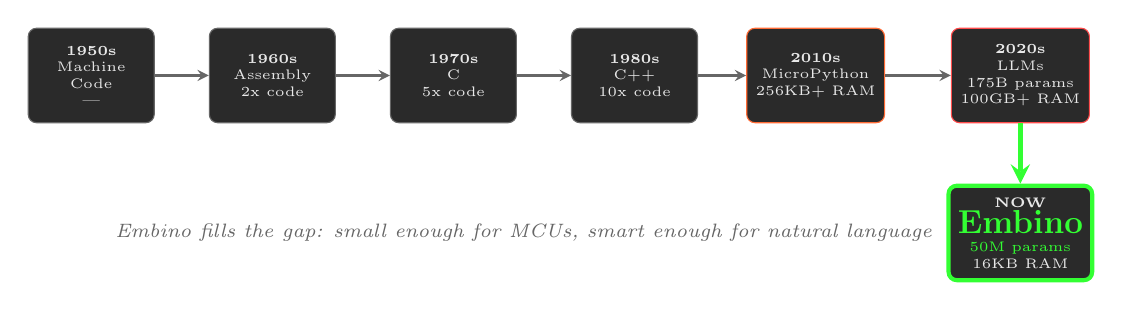
\begin{tikzpicture}[
    box/.style={draw, rounded corners=3pt, minimum width=1.6cm, minimum height=1.2cm, align=center, font=\tiny, text=termwhite},
    pastbox/.style={box, draw=termgray, fill=termdarkgray},
    pythonbox/.style={box, draw=termorange, fill=termdarkgray},
    llmbox/.style={box, draw=red!70, fill=termdarkgray},
    embinobox/.style={box, draw=termgreen, fill=termdarkgray, line width=1.5pt},
    arrow/.style={->, >=stealth, termgray, thick}
]

% Row 1: Historical
\node[pastbox] (mc) at (0,0) {\textbf{1950s}\\Machine\\Code\\---};
\node[pastbox] (asm) at (2.3,0) {\textbf{1960s}\\Assembly\\2x code};
\node[pastbox] (c) at (4.6,0) {\textbf{1970s}\\C\\5x code};
\node[pastbox] (cpp) at (6.9,0) {\textbf{1980s}\\C++\\10x code};

\draw[arrow] (mc) -- (asm);
\draw[arrow] (asm) -- (c);
\draw[arrow] (c) -- (cpp);

% Row 2: Python + LLM
\node[pythonbox] (py) at (9.2,0) {\textbf{2010s}\\MicroPython\\256KB+ RAM};
\node[llmbox] (llm) at (11.8,0) {\textbf{2020s}\\LLMs\\175B params\\100GB+ RAM};

\draw[arrow] (cpp) -- (py);
\draw[arrow] (py) -- (llm);

% Embino - below, with arrow down
\node[embinobox] (embino) at (11.8,-2) {\textbf{NOW}\\\large\textbf{\color{termgreen}Embino}\\[0.1em]\color{termgreen}50M params\\16KB RAM};

\draw[->, >=stealth, termgreen, line width=2pt] (llm.south) -- (embino.north);

% Gap annotation
\node[font=\scriptsize, color=termgray] at (5.5,-2) {\textit{Embino fills the gap: small enough for MCUs, smart enough for natural language}};

\end{tikzpicture}
\end{center}

\vspace{-0.3em}

% RAM bar chart (dark theme)
\begin{center}
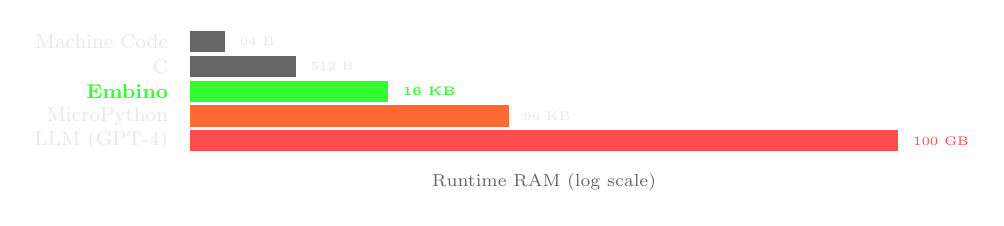
\begin{tikzpicture}[scale=0.9, every node/.style={scale=0.9}]
\footnotesize

\def\barheight{0.35cm}

% Labels and bars (ordered: Machine Code < C < Embino < MicroPython < LLM)
\node[anchor=east, text=termwhite] at (-0.2, 2.5*\barheight) {Machine Code};
\node[anchor=east, text=termwhite] at (-0.2, 1.5*\barheight) {C};
\node[anchor=east, text=termgreen, font=\footnotesize\bfseries] at (-0.2, 0.5*\barheight) {Embino};
\node[anchor=east, text=termwhite] at (-0.2, -0.5*\barheight) {MicroPython};
\node[anchor=east, text=termwhite] at (-0.2, -1.5*\barheight) {LLM (GPT-4)};

% Bars (log-scaled visually)
\fill[termgray] (0, 2.5*\barheight-0.15cm) rectangle (0.5cm, 2.5*\barheight+0.15cm);
\fill[termgray] (0, 1.5*\barheight-0.15cm) rectangle (1.5cm, 1.5*\barheight+0.15cm);
\fill[termgreen] (0, 0.5*\barheight-0.15cm) rectangle (2.8cm, 0.5*\barheight+0.15cm);
\fill[termorange] (0, -0.5*\barheight-0.15cm) rectangle (4.5cm, -0.5*\barheight+0.15cm);
\fill[red!70] (0, -1.5*\barheight-0.15cm) rectangle (10cm, -1.5*\barheight+0.15cm);

% Values
\node[anchor=west, font=\tiny, text=termwhite] at (0.6cm, 2.5*\barheight) {64 B};
\node[anchor=west, font=\tiny, text=termwhite] at (1.6cm, 1.5*\barheight) {512 B};
\node[anchor=west, font=\tiny\bfseries, text=termgreen] at (2.9cm, 0.5*\barheight) {16 KB};
\node[anchor=west, font=\tiny, text=termwhite] at (4.6cm, -0.5*\barheight) {96 KB};
\node[anchor=west, font=\tiny, text=red!70] at (10.1cm, -1.5*\barheight) {100 GB};

\node[anchor=north, font=\scriptsize, text=termgray] at (5cm, -2.5*\barheight) {Runtime RAM (log scale)};
\end{tikzpicture}
\end{center}

\cvsection{Why Now / Competitive Moat}

\begin{cvparagraph}
\textbf{\color{termcyan}Why now:} Grammar-constrained decoding and efficient LoRA adaptation only became viable in 2023-24. Small language models (<100M params) now match GPT-3 on structured tasks. The timing is right.

\textbf{\color{termorange}Competition:} MicroPython (too heavy, 96KB+), block-based tools (no AI, fixed templates), cloud LLMs (can't run on MCU). No one combines NL→DSL→verified bytecode→deterministic MCU execution.

\textbf{\color{termgreen}Moat:} 35-claim patent covering the full stack. First-mover in grammar-constrained embedded code generation.
\end{cvparagraph}

\cvsection{Market \& Business Plan}

\begin{cvparagraph}
\textbf{\color{termwhite}Market:} 30+ billion MCUs ship annually—all programmed in C/C++. Target: makers/education → robotics/automation → industrial OEMs. Even 0.1\% = 30M+ units/year.

\textbf{\color{termwhite}Business model:} Toolchain licenses (freemium → pro), dev board sales, OEM licensing fees for embedded runtime.

\textbf{\color{termcyan}Three-Stage Roadmap:}
\textbf{Stage 1} (12-24mo): Add-on module via UART/I²C for existing boards. Dev boards, makers, schools.
\textbf{Stage 2} (24-36mo): System-on-PCB with integrated interpreter. Volume sales, robotics kits.
\textbf{Stage 3} (36mo+): Custom SoC with ROM-resident runtime. OEM licensing.
\end{cvparagraph}

\cvsection{Investment Opportunity}

\begin{cvparagraph}
\textbf{\color{termgreen}Seeking \$500K seed round} to build production toolchain and Stage 1 hardware prototype.

\textbf{Use of funds:} DSL spec + reference interpreter, GC-SLM translator, micro-VM firmware (ESP32/Arduino/RP2040), first add-on module design, partner outreach.

• \textbf{\color{termgreen}Product-first:} Real toolchain for real hardware—not a research benchmark\\
• \textbf{\color{termgreen}Strong IP:} 35-claim provisional patent covering the full stack\\
• \textbf{\color{termgreen}Massive market:} 30B+ MCUs/year still using 50-year-old programming\\
• \textbf{\color{termgreen}Founder fit:} 6 years embedded ML at Apple/Intel, 15 patents (depth sensing, ML, medical imaging), startup exit, Nature publication
\end{cvparagraph}

\end{document}

